\documentclass[12pt,a4paper]{article}

\usepackage{graphicx}
\usepackage{hyperref}
\usepackage{amsmath}
\usepackage[margin=1in]{geometry}

\title{Image Inpainting with Deep Learning}
\author{Ian Li \\ Harvey Mudd College}
\date{}

\begin{document}

\maketitle

\begin{abstract}
This report delves into the exploration of image inpainting using deep learning techniques. Image inpainting, the process of reconstructing missing or damaged areas of digital images, is a crucial task in various domains such as photo enhancement, restoration of historical images, and content editing. Traditional methods, while effective to a degree, face limitations in handling complex textures or large missing regions. This study investigates the efficacy of convolutional autoencoders and partial convolutions in addressing these challenges, utilizing the CIFAR10 dataset for experimentation.
\end{abstract}

\section{Introduction}

\subsection{Overview of Image Inpainting}
Image inpainting is a sophisticated technique aimed at filling in missing or damaged areas of digital images. The core purpose of image inpainting includes enhancing photo quality, restoring historical images, and editing content within images. The need for advanced inpainting methods has grown with the digital age, as more sophisticated and seamless restoration becomes possible and desirable.

\subsection{Traditional Image Inpainting Methods}
Traditionally, image inpainting has relied on patch-based methods, where patches from the surrounding areas are utilized to fill in gaps. However, these methods often fall short when the surrounding regions lack suitable information or when the missing regions are too large or complex, necessitating the inpainting system to infer properties of the would-be-present objects. It is in these scenarios that deep learning approaches show promise, with the ability to capture and utilize spatial contexts within images more effectively.

\section{Data}

\subsection{CIFAR10 Dataset}
The CIFAR10 dataset is a cornerstone in machine learning research, consisting of 60,000 32x32 color images categorized into 10 classes. It serves as a benchmark for comparing the effectiveness of different machine learning methods and has been pivotal in tracking progress in the field.

\begin{center}
	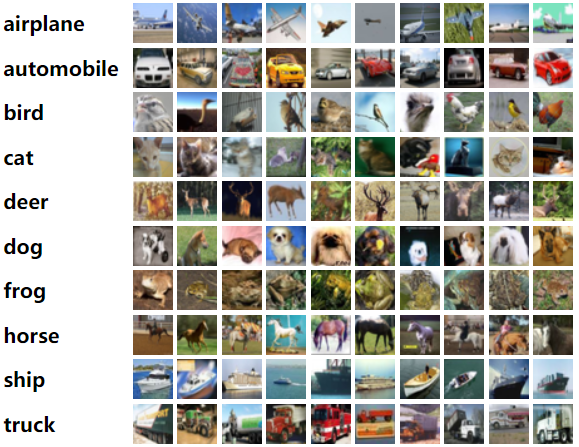
\includegraphics[scale=0.5]{cifar10.png}
\end{center}

\subsection{Data Preparation}
To simulate the conditions for image inpainting, the study introduces artificial deterioration to the images in the CIFAR10 dataset. This is achieved by using OpenCV to draw lines of random length and thickness over the images, thereby creating masks that simulate missing or damaged sections of the images.

\begin{center}
	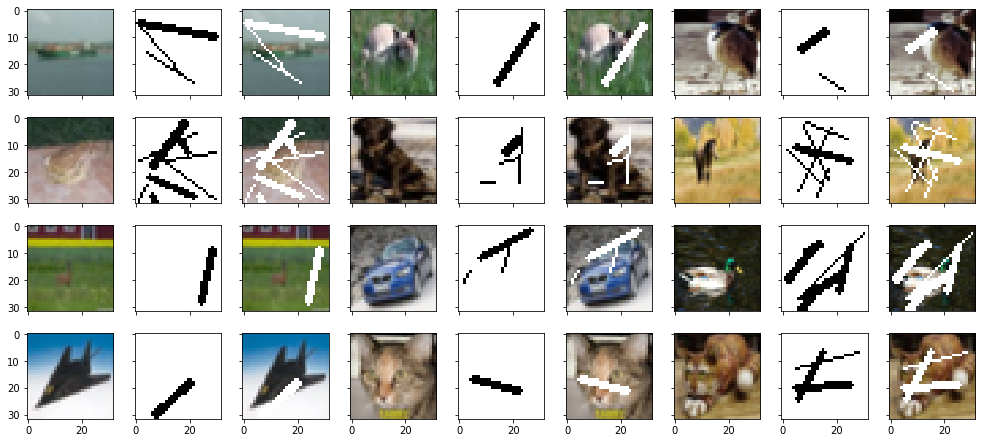
\includegraphics[scale=0.5]{masks.png}
\end{center}
\section{Methods}

\subsection{Convolutional Autoencoders}
Convolutional autoencoders are neural networks designed to learn a compressed, yet comprehensive representation of a dataset. The encoder component of an autoencoder reduces the input data to a lower-dimensional representation, which the decoder component then uses to reconstruct the original data. The use of convolutions allows the network to learn hierarchical representations of data, including shapes, edges, and textures, which are crucial for effective image inpainting.
\begin{center}
	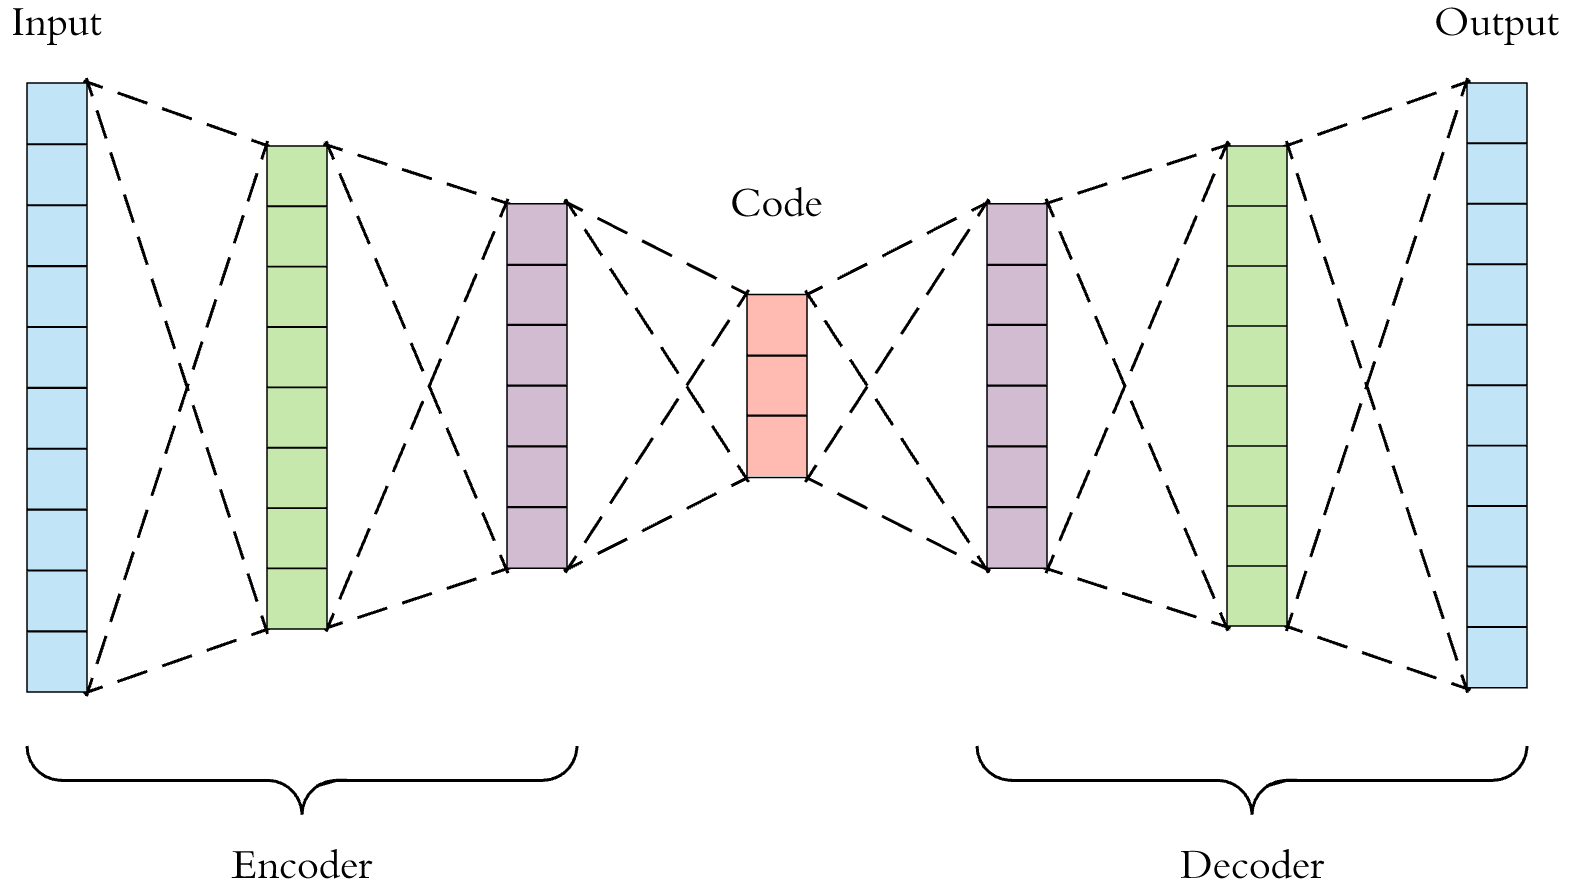
\includegraphics[scale=0.2]{autoencoder.png}
\end{center}

\subsection{Partial Convolutions}
Partial convolutions offer a solution to the limitation of traditional convolutional layers, which use missing pixels in their computations, often leading to poor image quality. By focusing solely on valid pixels for learning representations and updating the mask after each partial convolution operation, partial convolutions aim to produce higher quality inpainted images.
\begin{center}
	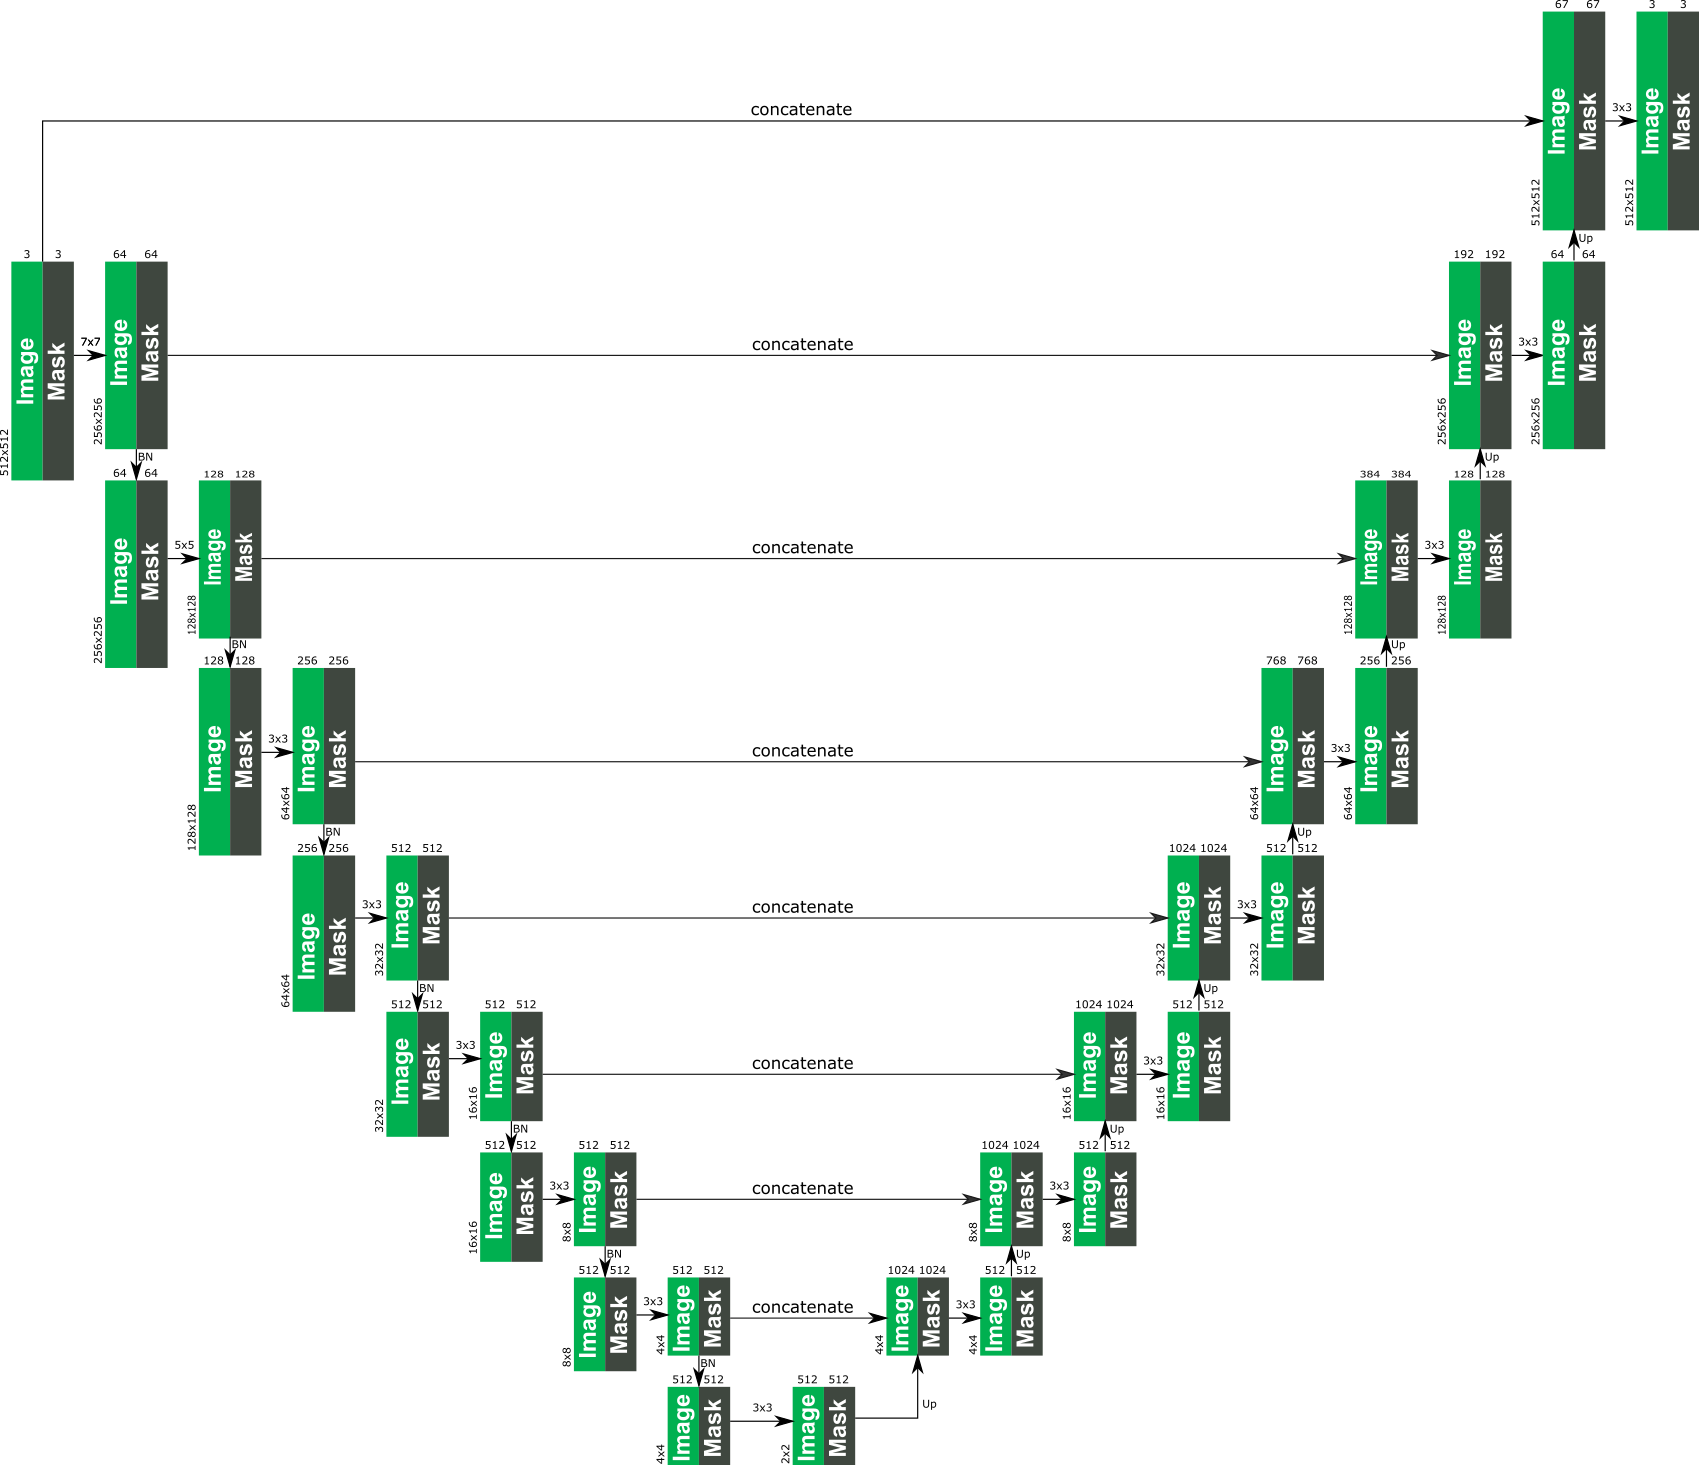
\includegraphics[scale=0.2]{partial3.png}
\end{center}
\section{Results}

\subsection{Convolutional Autoencoder Results}
The convolutional autoencoder showed promising results, with the reconstructed images displaying considerable improvements over the masked inputs. However, some artifacts were still present, indicating room for refinement.

\begin{center}
	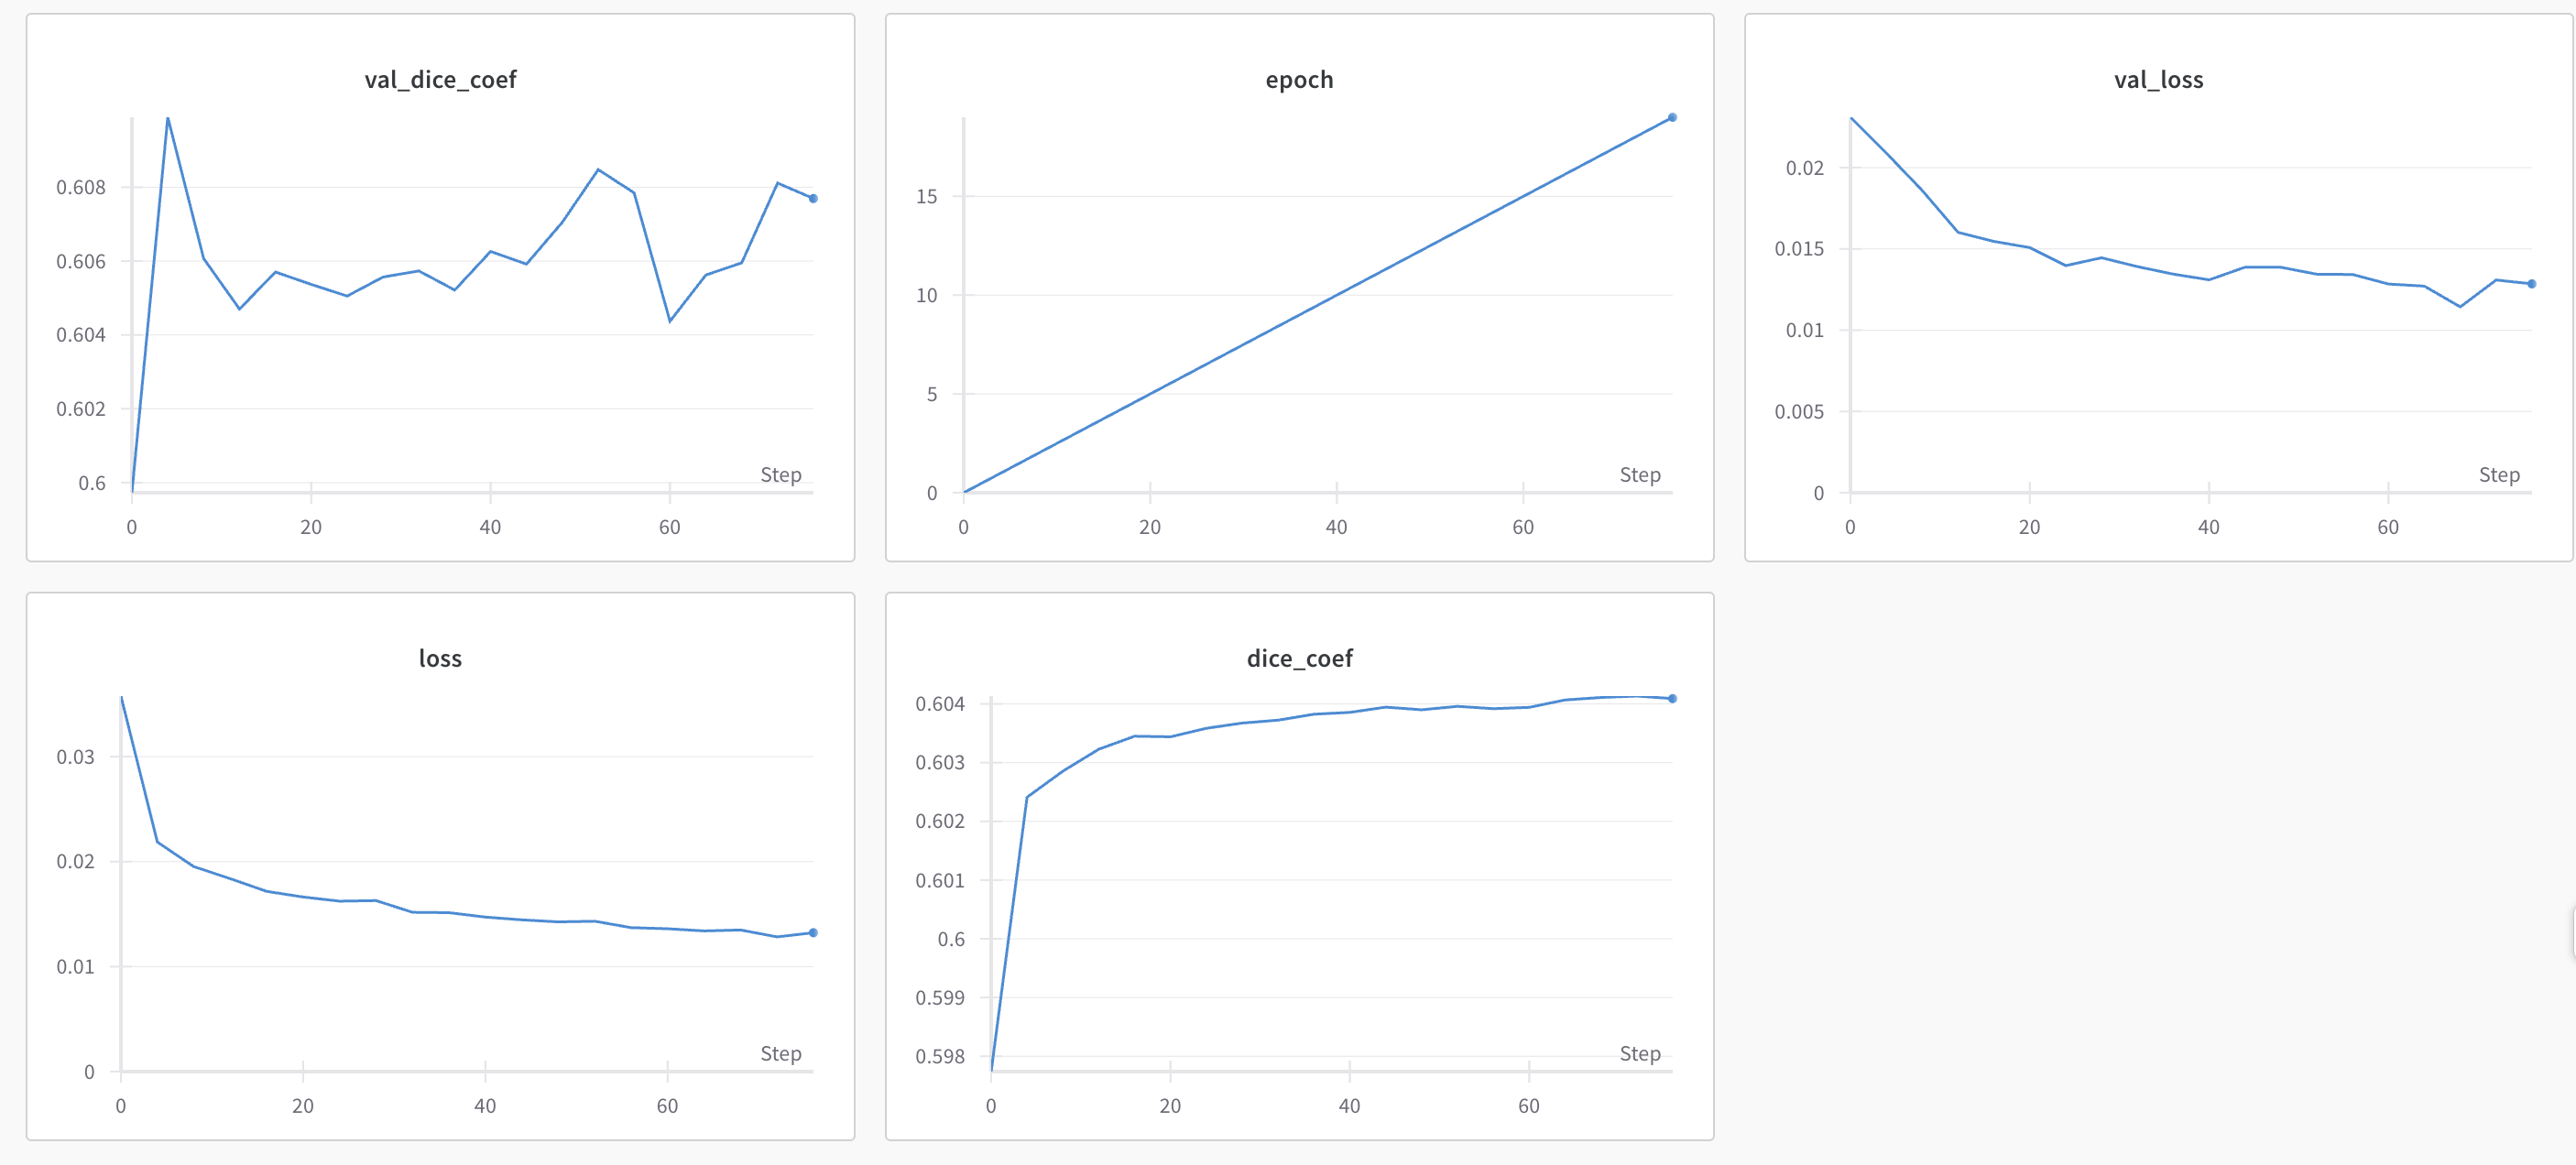
\includegraphics[scale=0.3]{result1.png}
\end{center}

\subsection{Partial Convolutional Autoencoder Results}
It can be observed that the traditional CNN-based approach to image inpainting yielded slightly better results compared to the method utilizing partial convolutions. This outcome primarily stems from the complexity of the partial convolution architecture when applied to the CIFAR10 dataset. Partial convolution layers are specifically engineered for high-resolution images, typically those exceeding 256x256 pixels in size, which explains the discrepancy in performance.

\begin{center}
	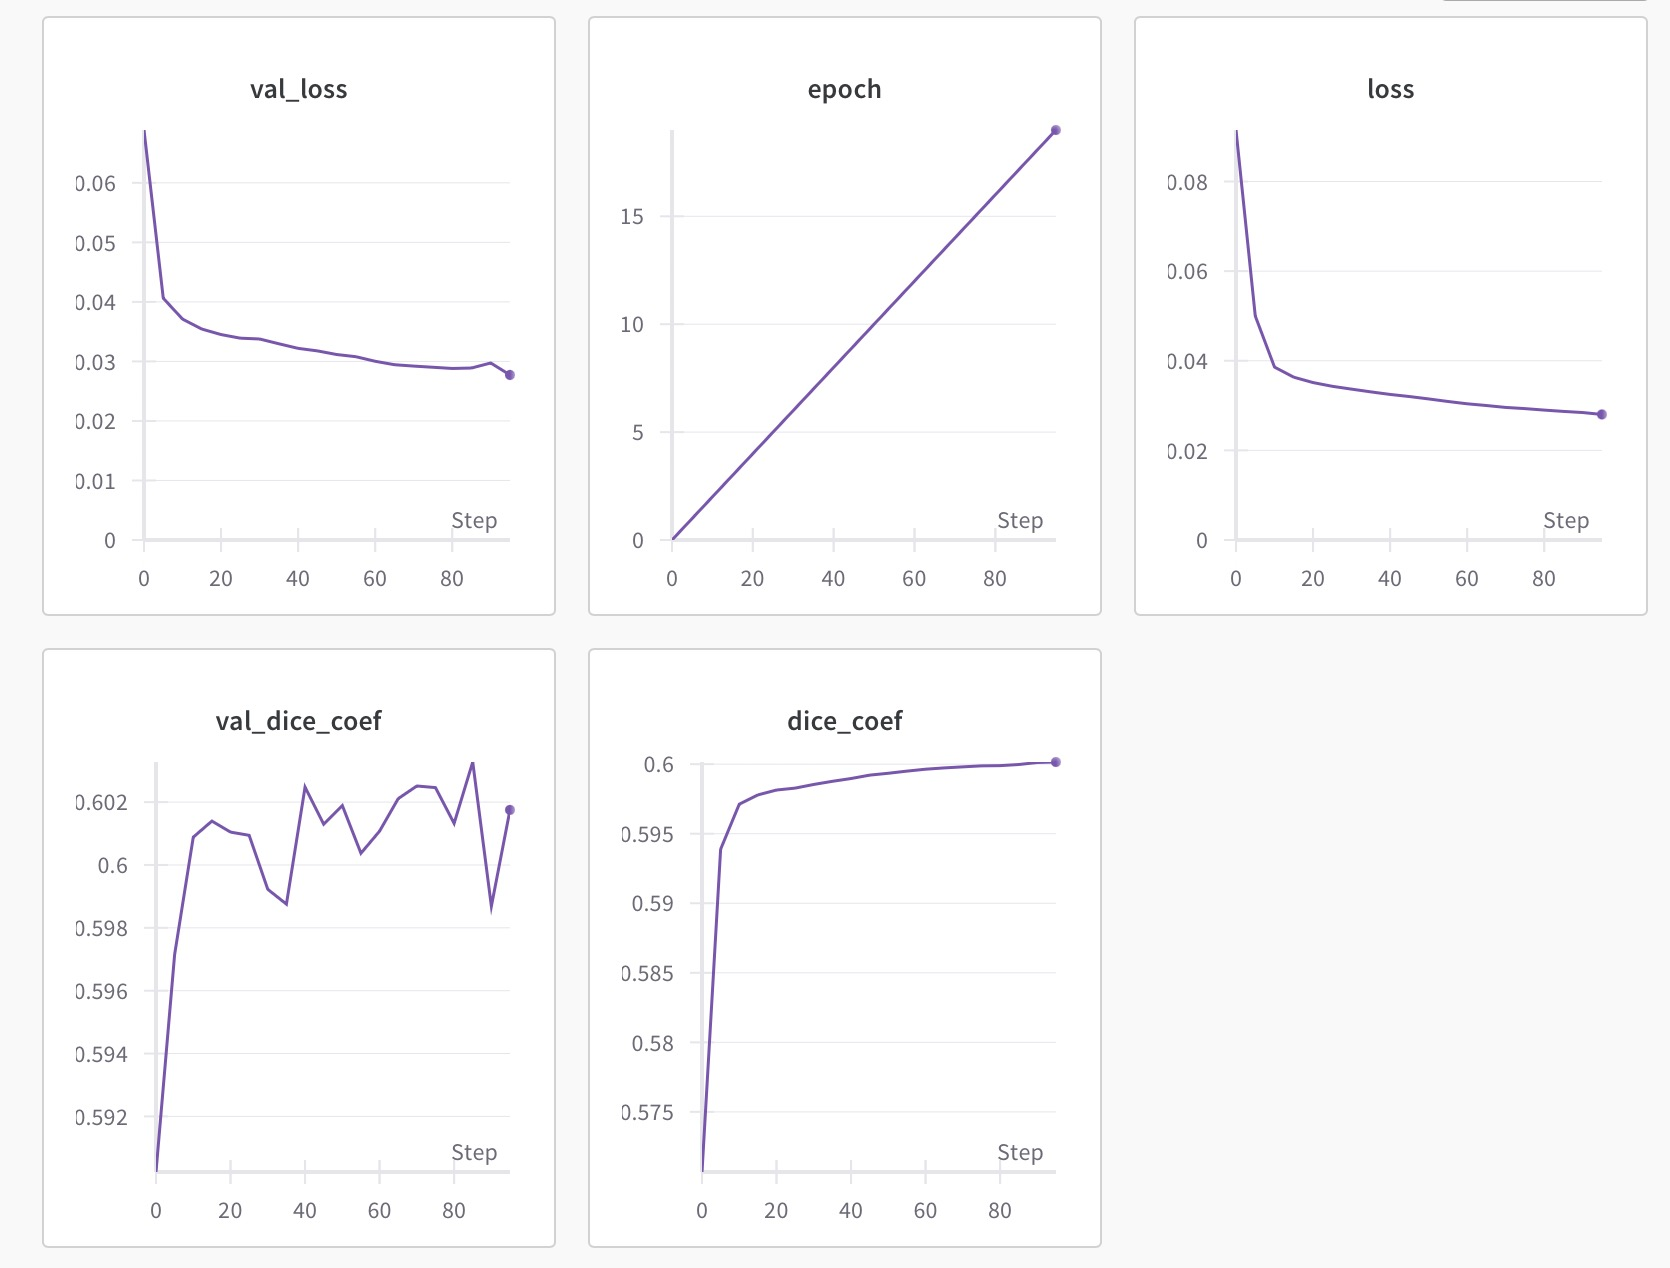
\includegraphics[scale=0.4]{results2.jpg}
\end{center}

\section{Next Steps}
The next phase of this research will focus on testing both the convolutional autoencoder and partial convolutional autoencoder methods on higher resolution datasets. Additionally, the potential of integrating image inpainting with stable diffusion models will be explored, examining the tractability of diffusion models in this context.

\section*{References}
\begin{enumerate}
    \item CIFAR-10 - Learning Multiple Layers of Features from Tiny Images, Alex Krizhevsky, 2009.
    \item Image Inpainting for Irregular Holes Using Partial Convolutions, Guilin Liu et al., 2018.
    \item Auto-Encoding Variational Bayes, Kingma and Welling, 2013.
\end{enumerate}

\end{document}
